
\newcommand*\plusc{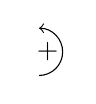
\begin{tikzpicture} \draw[->] (0,-1) arc (-90:90:0.3) node[left,pos=0.5,xshift=2] {\(+\)};\end{tikzpicture}}

\item Se tiene un resorte de largo natural $l_0$ el cual se encuentra unido a una barra de masa despreciable, con una masa $m$ puntual en su extremo, como se muestra en la figura.

\begin{enumerate}[a)]
	\item Si la barra pivotea en $O$, determine lo que se deforma el resorte si la posición de equilibrio del sistema corresponde a la horizontal.
	\item Si el sistema se saca levemente de su posición de equilibrio, obtener la ecuación de movimiento para la variable $\theta$ y la frecuencia angular para pequeñas oscilaciones. La variable $\theta$ se mide desde la horizontal de la barra y a favor de las manecillas del reloj.
	\item Considere ahora el mismo problema pero en presencia de una fuerza de amortiguación aplicada en la masa $m$ tangente al movimiento. Si en $t=0$, el sistema se saca del equilibrio un ángulo $\theta_0$. Obtenga la solución para $t>0$. Calcule el tiempo para el cual la amplitud ha disminuido a la décima parte de su amplitud inicial.
	\item Considere una situación en que una fuerza dependiente del tiempo de forma sinusoidal golpea a la masa de forma tangente al movimiento. Calcule el promedio de la energía para un periodo de tiempo en estado estacionario. Obtenga la frecuencia para la cual la energía se hace máxima.
	\begin{equation*}
		\bar{E} = \dfrac{1}{T} \int_0^T E(t) \ dt \hspace{10mm} (T \equiv \text{periodo})
	\end{equation*}
\end{enumerate}

\begin{figure}[h]
	\centering
	\fbox{
		\begin{tikzpicture}[scale=1]
		\draw [very thick] (0,-0.75) -- (2,-0.75);
		\draw [decoration={aspect=0.3, segment length=1.5mm, amplitude=4mm,coil},decorate] (1,-0.75) -- (1,-2.5);
		\node at (-.3,-1.5) {\(k\)};
		\fill [pattern = north east lines] (0,-.55) rectangle (2,-0.75);
		\draw [<->,thick] (2,-.75) -- (2,-2.5) node [right,midway] {\(l_0\)};	
		
		\draw [dashed] (.5,-2.5) -- (7.5,-2.5);
		
		\draw [very thick] (6,-0.75) -- (8,-0.75);
		\draw [decoration={aspect=0.3, segment length=1.5mm, amplitude=4mm,coil},decorate] (7,-0.75) -- (7,-3);
		\fill [pattern = north east lines] (6,-.55) rectangle (8,-0.75);
		\draw [<->,thick] (8,-.75) -- (8,-3) node [right,midway] {\(l\)};
		\draw (4,-3) rectangle (10,-3.4);
		\draw [<->,thick] (4,-3.8) -- (10,-3.8) node [below,midway] {\(L\)};
		\draw [fill=black] (10,-3.2) circle (2mm);
		\node at (10.5,-3.2) {\(m\)};
		\draw [fill=white] (4,-3.2) circle (.5mm);
		\node at (3.7,-3.2) {\(O\)};
		\end{tikzpicture}}
\end{figure}

\underline{\textbf{Solución:}}

%FinEnuc

\begin{enumerate}[a)]
	
	\item El DCL de la barra es el siguiente:
	\begin{figure}[H]
		\centering
		\begin{tikzpicture}[scale=1.5]
			\draw[red,->] (-1,0) -- (0,0) node [pos=0.1,above] {\(R_\text{x}\)};
			\draw[black,ultra thick] (0.05,0) -- (4,0);
			\draw[red,->] (4,-0.05) -- (4,-1) node [right] {\(mg\)};
			\draw[red,->] (0.05,0.05) -- (0.05,1) node[right] {\(R_\text{y}\)};
			\draw[red,->] (2,0.05) -- (2,1) node[right] {\(F_\text{R}\)};
		\end{tikzpicture}
	\end{figure}
	Aplicando torque respecto al punto $O$:
	\begin{equation*}
		\sum \tau_0 = F_{\text{R}} \frac{L}{2} - mgL = 0 \Rightarrow F_\text{R} = 2mg
	\end{equation*} 
	La deformación del resorte $\Delta y$ se puede expresar como:
	\begin{equation*}
	\tcbhighmath{\Delta y = \frac{2mg}{k}}
	\end{equation*}
	
	\item A continuación se muestra el DCL de la barra con la variable $\theta$:
	\begin{figure}[H]
		\centering
		\begin{tikzpicture}[scale=1.5]
		\begin{scope}[rotate=-30]
		\draw[black,ultra thick] (0.05,0) -- (4,0);
%		\draw[dashed] (2,0) -- (2,0.95) node [midway,left,scale=0.8,xshift=2] {\( \theta \)};
%		\draw[dashed] (4,0) -- (4,-0.95) node [pos=0.6,right,scale=0.8,xshift=-2] {\( \theta \)};
		\end{scope}
		\draw[red,->] (0.05,0.05) -- (0.05,1) node[right] {\(R_\text{y}\)};
		\draw[dashed] (0.05,0) -- (1.3,0) node[below,midway,scale=0.8,yshift=0] {\(\theta\)};
		\draw[red,->] (1.7,-.95) -- (1.7,0) node[above] {\(F_\text{R}\)};
		\draw[red,->] (-1,0) -- (0,0) node [pos=0.1,above] {\(R_\text{x}\)};
		\draw[red,->] (3.45,-2.05) -- (3.45,-3.05) node [right] {\(mg\)};
		\end{tikzpicture}
	\end{figure}
	Aplicando torque respecto al punto $O$:
	\begin{equation*}
		\sum \tau_0 = I\ddot{\theta} = mgL\cos \theta - k \dfrac{L}{2} \left( \dfrac{2mg}{k} + \dfrac{L}{2} \sin \theta \right)
	\end{equation*}
	El momento de inercia es $I = mL^2$. Por lo tanto, la ecuación de movimiento es para oscilaciones pequeñas es:
	\begin{equation*}
	\tcbhighmath{\ddot{\theta}+\frac{k}{4m}\theta = 0}
	\end{equation*}
	La frecuencia angular natural del sistema $\omega_0$ es:
	\begin{equation*}
	\tcbhighmath{\omega_0 = \sqrt{\frac{k}{4m}}}
	\end{equation*}
	
	\item La fuerza de amortiguación $F_{\text{a}}$ está dada por $F_{\text{a}} = b \dot{S}$, donde $S = L \theta$.
	
	\begin{figure}[H]
		\centering
		\begin{tikzpicture}[scale=1.5]
			\begin{scope}[rotate=-20]
				\draw[black,ultra thick] (0.05,0) -- (4,0);
				\draw[->,red] (4,0.05) -- (4,1) node[right,midway] {$F_{\text{a}}$};
			\end{scope}
			
			\draw[red,->] (0.05,0.05) -- (0.05,1) node[right] {\(R_{\text{y}}\)};
			\draw[red,->] (1.8,-.6) -- (1.8,0.4) node[right] {\(F_{\text{R}}\)};
			\draw[red,->] (-1,0) -- (0,0) node [pos=0.1,above] {\(R_{\text{x}}\)};
			\draw [red,->] (3.75,-1.4) -- (3.75,-2.4) node[right] {\( mg \)};
		\end{tikzpicture}
	\end{figure}
	\begin{equation*}
	\sum \tau_0 = I\ddot{\theta} = mgL\cos \theta - k \dfrac{L}{2} \left( \dfrac{2mg}{k} + \dfrac{L}{2} \sin \theta \right) - b \dot{S} L
	\end{equation*}
	Considerando $\dot{S} = L \dot{\theta}$, la ecuación de movimiento es:
	\begin{equation*}
	\tcbhighmath{	\ddot{\theta} + \dfrac{b}{m} \dot{\theta} + \frac{k}{4m} \ \theta = 0}
	\end{equation*}
	La solución es de la forma:
	\begin{equation*}
		\theta(t) = A e^{-\gamma t} \cos (\omega t + \phi)
	\end{equation*}
	\noindent donde $\omega^2 = \omega_0^2 - \gamma^2$ y $\gamma = \frac{b}{2m}$. $A$ y $\phi$ se obtienen con las condiciones iniciales del sistema, $\theta(0) = A \cos (\phi) = \theta_0$.
	\begin{equation*}
		\theta(t) = \dfrac{\theta_0}{\cos \phi} e^{-\gamma t} \cos (\omega t + \phi)
	\end{equation*}
	El tiempo para el cual la amplitud ha disminuido a la décima parte de su amplitud inicial es:
	\begin{equation*}
		\dfrac{1}{10} \dfrac{\theta_0}{\cos \phi} = \dfrac{\theta_0}{\cos \phi} e^{-\frac{b}{2m} t}
	\end{equation*}
	\begin{equation*}
		\tcbhighmath{t = \dfrac{2m}{b} \ln 10 = \dfrac{\ln 10}{\gamma}}
	\end{equation*}

	\item La fuerza externa está dada por $F_\text{ext} = F_0 \cos (\Omega t)$. Aplicando la fuerza externa a la ecuación de movimiento se obtiene:
	\begin{align*}
	\sum \tau_0 = I\ddot{\theta} = mgL\cos \theta - k \dfrac{L}{2} \left( \dfrac{2mg}{k} + \dfrac{L}{2} \sin \theta \right) - b \dot{S} L + F_{\text{ext}}L
	\end{align*}
	\begin{align*}
	\tcbhighmath{\ddot{\theta} + \dfrac{b}{m} \dot{\theta} + \frac{k}{4m} \ \theta = \dfrac{F_0}{mL} \cos (\Omega t)}
	\end{align*}
	La solución para régimen estacionario es $\theta(t) = A_2 \cos (\omega t + \phi)$. La energía del sistema está dada por:
	\begin{align*}
	E(t) = \dfrac{1}{2} I \dot{\theta}^2 + \dfrac{1}{2} k x^2 + mgh
	\end{align*}
	
\end{enumerate}
